\chapter{Especiación y macroevolución}\label{ch:b2:speciation}

En una pequeña isla de las Galápagos, en 1982, llegaron unos pocos
pinzones terrestres grandes procedentes de una isla vecina y se quedaron.
Durante veinte años compitieron con el pinzón terrestre mediano residente
por las \omterm{def:b2:angiosperm-reproduction:seed}{semillas} grandes que ambos preferían; después llegó una sequía,
las \omterm{def:b2:angiosperm-reproduction:seed}{semillas} grandes escasearon, y los residentes de pico más grande ---
los que competían más directamente con los recién llegados --- murieron de
hambre. En una sola generación, los picos de los residentes se habían
reducido, de forma medible, alejándose de los de los invasores. Dos
especies que se habían encontrado fueron empujadas en sentidos opuestos.
Este capítulo trata de la formación de las especies: qué es una especie y
qué la mantiene distinta, cómo una población se convierte en dos, la
competencia que separa a las poblaciones cuando se encuentran, y la visión
a largo plazo del registro fósil, donde el mismo proceso repetido más de
cien millones de veces da el árbol de la vida.

\section{Qué es una especie}

\begin{definition}[Especie]\label{def:b2:speciation:species}
\index{concepto de especie}\index{concepto biológico de especie}\index{aislamiento reproductivo}
Según el \emph{concepto biológico de especie}, una especie es un grupo de
poblaciones cuyos miembros pueden cruzarse entre sí y producir
descendencia fértil, y que están \emph{aisladas reproductivamente} de los
demás grupos de ese tipo: lo que une a una especie es el \omterm{prop:b2:population-genetics:migration}{flujo génico}, y
lo que separa a las especies es su ausencia. El concepto funciona para los
organismos sexuados de un tiempo y un lugar, que son la mayor parte de lo
que encuentra un biólogo; falla para los linajes asexuales (que se
nombran por su parecido), para los fósiles (que no pueden cruzarse) y para
los numerosos casos en que la frontera deja pasar genes --- robles y
sauces que se hibridan entre especies, patos cuyas especies se cruzan en
cautividad, especies en anillo en las que las poblaciones vecinas se
cruzan a lo largo de todo el contorno de una barrera hasta que los
extremos se encuentran y ya no lo hacen. Otros conceptos llenan los
huecos: la especie \emph{morfológica} (un conjunto de formas parecidas),
la \emph{filogenética} (el menor linaje diagnosticable), la
\emph{ecológica} (un linaje que ocupa su propio nicho). Ninguno es
erróneo; cada uno mide algo real, y la especiación es el proceso por el
que acaban coincidiendo.
\end{definition}

\begin{proposition}[Mecanismos de aislamiento]\label{prop:b2:speciation:isolation}
\index{mecanismo de aislamiento}\index{aislamiento precigótico}\index{aislamiento poscigótico}\index{regla de Haldane}
El \omterm{prop:b2:population-genetics:migration}{flujo génico} entre dos poblaciones se detiene por barreras que actúan
antes o después de la fecundación. \emph{Precigóticas}: las poblaciones
viven en hábitats distintos o se reproducen en estaciones distintas
(aislamiento temporal: dos ranas que cantan en meses distintos); no
reconocen el cortejo de la otra (comportamental: los cantos de los grillos,
los códigos luminosos de las luciérnagas, las danzas de los patos); sus
genitales o sus \omterm{def:b2:angiosperm-reproduction:flower}{flores} no encajan (mecánico); sus gametos no se fusionan
(gamético: las proteínas de unión del espermatozoide de los erizos de mar,
los \omterm{def:b2:meiosis-heredity:vocabulary}{alelos} $S$ del \cref{ch:b2:angiosperm-reproduction}).
\emph{Poscigóticas}: el híbrido muere como embrión, o vive pero es estéril
(la mula; los híbridos de dos especies de \emph{Drosophila}), o es fértil
pero su propia descendencia no lo es (degradación híbrida).
\emph{\omterm{prop:b2:speciation:isolation}{Regla de Haldane}}: cuando solo un sexo de un híbrido es estéril o
inviable, es el sexo con dos \omterm{prop:b2:meiosis-heredity:sexlinked}{cromosomas sexuales} distintos --- el macho en
los mamíferos y las moscas, la hembra en las aves y las mariposas ---,
porque las incompatibilidades recesivas del X quedan expuestas en él. Las
barreras precigóticas son más baratas, puesto que no se desperdician
gametos, y la selección las construye allí donde ya existen las
poscigóticas.
\end{proposition}

\begin{theorem}[Por qué fracasan los híbridos: el modelo de dos loci]\label{thm:b2:speciation:dm}
\index{incompatibilidad de Dobzhansky--Muller}
Dos poblaciones parten del \omterm{def:b2:meiosis-heredity:vocabulary}{genotipo} $aabb$. En una, $a$ es sustituido
por $A$; en la otra, $b$ por $B$; cada sustitución es neutra o favorable
en su propio fondo genético, de modo que ninguna población pasa nunca por
un estado menos apto. Pero $A$ y $B$ nunca se han puesto a prueba juntos,
y si la combinación es incompatible --- si la proteína que fabrica $A$ no
puede funcionar con la proteína que fabrica $B$ ---, el híbrido $AaBb$ es
poco apto. El \omterm{def:b2:speciation:species}{aislamiento reproductivo} surge así como subproducto de la
divergencia, sin cruzar ningún valle y sin selección a favor del
aislamiento en sí; y como cada nueva sustitución en un linaje puede ser
incompatible con cada sustitución ya fijada en el otro, el número de
incompatibilidades posibles crece como el
\emph{cuadrado} del número de sustituciones --- el aislamiento crece
\emph{como una bola de nieve} con el tiempo.
\end{theorem}
\begin{proof}
Con $n$ sustituciones en cada linaje, cada uno de los $n$ \omterm{def:b2:meiosis-heredity:vocabulary}{alelos} nuevos de
un linaje puede ser incompatible con cada uno de los $n$ del otro:
$n^{2}$ pares, cada uno incompatible con cierta probabilidad
$\varepsilon$, de modo que el número esperado de incompatibilidades es
$\varepsilon n^{2}$, y $n$ crece con el tiempo transcurrido desde la
separación. El híbrido es el único \omterm{def:b2:meiosis-heredity:vocabulary}{genotipo} en el que se encuentran los
dos conjuntos.
\end{proof}
\begin{proof}[Evidencia]
Coyne y Orr (1989, 1997) reunieron cientos de pares de especies de
\emph{Drosophila} de distancia genética conocida (una medida del tiempo
transcurrido desde la divergencia) y midieron su \omterm{prop:b2:speciation:isolation}{aislamiento precigótico} y
poscigótico: ambos aumentan con la distancia, el aislamiento es
prácticamente completo a una distancia que corresponde a unos pocos
millones de años, y los pares que viven en la misma región muestran, a
igual distancia, un \omterm{prop:b2:speciation:isolation}{aislamiento precigótico} más fuerte que los que no ---
la huella del refuerzo. Desde entonces se han identificado uno a uno genes
de incompatibilidad, y el número hallado entre dos especies crece, en
efecto, más deprisa que linealmente con su divergencia.
\end{proof}
\begin{omfigure}
\begin{tikzpicture}[every node/.style={font=\scriptsize}, >=stealth]
  \node[draw, rounded corners, fill=omExo!25] (anc) at (0,0) {antepasado $aabb$};
  \node[draw, rounded corners, fill=omDef!15] (p1) at (-2.6,-1.8) {población 1: $AAbb$};
  \node[draw, rounded corners, fill=omThm!15] (p2) at (2.6,-1.8) {población 2: $aaBB$};
  \node[draw, rounded corners, fill=gray!25, align=center] (hyb) at (0,-3.6) {híbrido $AaBb$:\\$A$ y $B$ se encuentran por primera vez\\--- incompatibles, poco apto};
  \draw[->, thick] (anc) -- (p1) node[midway, left, align=right] {$a \to A$ fijado,\\apto en su fondo};
  \draw[->, thick] (anc) -- (p2) node[midway, right, align=left] {$b \to B$ fijado,\\apto en su fondo};
  \draw[->, thick] (p1) -- (hyb); \draw[->, thick] (p2) -- (hyb);
  \node[anchor=west, align=left, text width=4.6cm] at (4.6,-0.4) {ninguna población cruzó un valle; el aislamiento es un subproducto, y el número de pares así crece como $n^{2}$};
\end{tikzpicture}

{\small El modelo de dos loci del fracaso de los híbridos. Cada población
fija un cambio que funciona en su propio fondo genético; el híbrido es el
primer \omterm{def:b2:meiosis-heredity:vocabulary}{genotipo} que combina los dos.}
\end{omfigure}

\section{Cómo una especie se convierte en dos}

\begin{proposition}[Modos de especiación]\label{prop:b2:speciation:modes}
\index{especiación alopátrica}\index{especiación simpátrica}\index{especiación parapátrica}\index{efecto fundador}
La especiación \emph{alopátrica} empieza con una barrera geográfica:
un área de distribución dividida por una montaña que se eleva, un mar que
se seca o un río nuevo (\emph{vicarianza}), o unos pocos colonos llevados a
una isla (\emph{peripátrica}, con el \omterm{prop:b2:speciation:modes}{efecto fundador} y la deriva del
\cref{ch:b2:population-genetics} añadidos). Aisladas del \omterm{prop:b2:population-genetics:migration}{flujo génico},
las dos poblaciones divergen por la selección en ambientes distintos, por
la deriva y por sus \omterm{def:b2:genome-diversification:mutation}{mutaciones} propias, hasta acumular
incompatibilidades; si vuelven a encontrarse, ya no se funden. Es el modo
más común, y la distribución de especies hermanas a ambos lados de cada
istmo, cordillera y estrecho es su registro. La especiación
\emph{simpátrica} se produce sin barrera: de un solo paso, por \omterm{def:b2:genome-diversification:polyploidy}{poliploidía}
(\cref{ch:b2:genome-diversification}) --- un tercio de las especies de
plantas surgió así ---, o por selección disruptiva con apareamiento
selectivo, cuando una población explota dos recursos y los individuos se
aparean sobre el recurso que usan (la mosca de la manzana, que pasó del
espino albar al manzano en la década de 1860 y ahora se aparea sobre su
hospedador; los cíclidos de un lago de cráter). La especiación
\emph{parapátrica} se produce a lo largo de un gradiente ambiental, donde
una población se adapta a los dos extremos y se forma una \omterm{prop:b2:speciation:reinforcement}{zona híbrida} en
el centro. En todos los modos la receta es la misma: reducir el \omterm{prop:b2:population-genetics:migration}{flujo
génico}, dejar que se acumule la divergencia y dejar que los subproductos
de la divergencia se conviertan en barreras.
\end{proposition}

\begin{omfigure}
\resizebox{\linewidth}{!}{%
\begin{tikzpicture}[every node/.style={font=\scriptsize}, >=stealth]
  \foreach \x/\lab in {0/{alopátrica:\\una barrera divide el área}, 5.2/{peripátrica:\\unos pocos fundadores en una isla}, 10.4/{simpátrica:\\dos hospedadores, apareamiento\\sobre el hospedador}} \node[align=center, anchor=south] at (\x+1.8,3.0) {\lab};
  % allopatric
  \draw[thick, fill=omDef!15] (0.9,1.4) ellipse (0.8 and 0.9);
  \draw[thick, fill=omThm!15] (2.7,1.4) ellipse (0.8 and 0.9);
  \draw[very thick, omExo!70!black] (1.8,0.2) -- (1.8,2.6);
  \node[below] at (1.8,0.1) {montaña, mar, río};
  % peripatric
  \begin{scope}[xshift=5.2cm]
    \draw[thick, fill=omDef!15] (1.0,1.4) ellipse (1.0 and 0.9);
    \draw[thick, fill=omThm!15] (3.2,1.9) circle (0.35);
    \draw[->, thick, dashed] (2.0,1.6) -- (2.85,1.85);
    \node[below] at (3.2,1.5) {fundadores};
    \node[below] at (1.0,0.4) {continente};
  \end{scope}
  % sympatric
  \begin{scope}[xshift=10.4cm]
    \draw[thick, fill=omExo!15] (1.8,1.4) ellipse (1.7 and 0.9);
    \foreach \p in {(1.0,1.6),(1.3,1.2),(0.8,1.2),(1.2,1.8)} \fill[omDef] \p circle (0.07);
    \foreach \p in {(2.4,1.6),(2.7,1.2),(2.2,1.2),(2.6,1.8)} \fill[omThm] \p circle (0.07);
    \node[omDef, below] at (1.0,0.5) {hospedador A}; \node[omThm, below] at (2.6,0.5) {hospedador B};
    \node[below] at (1.8,0.1) {un lugar, dos recursos};
  \end{scope}
\end{tikzpicture}}

{\small Tres caminos hacia dos especies: una barrera que atraviesa el área
de distribución, una población fundadora más allá de ella, o dos recursos
dentro de ella.}
\end{omfigure}

\begin{proposition}[Refuerzo y zonas híbridas]\label{prop:b2:speciation:reinforcement}
\index{refuerzo}\index{zona híbrida}\index{clina}
Cuando dos poblaciones que han divergido vuelven a encontrarse, pueden
ocurrir tres cosas. Si sus híbridos son tan aptos como los progenitores,
se funden. Si los híbridos son poco aptos, la selección favorece a los
individuos que rechazan aparearse con la otra forma --- el coste son los
gametos desperdiciados ---, y el \omterm{prop:b2:speciation:isolation}{aislamiento precigótico} se refuerza donde
las dos se superponen (\emph{refuerzo}), hasta que son especies. Entre
ambos casos persiste una
\emph{\omterm{prop:b2:speciation:reinforcement}{zona híbrida}}: una franja, a menudo de unos pocos kilómetros de
anchura, donde las dos formas se cruzan y se producen híbridos en cada
generación, mantenida por el equilibrio entre la dispersión hacia la zona
y la selección contra los híbridos dentro de ella. A través de una zona
así, la frecuencia de cada forma sigue una \emph{clina}, una curva en S
cuya anchura $w$ la fijan la distancia de dispersión $\sigma$ por
generación y la selección $s$ contra los híbridos, $w \approx
\sigma\sqrt{8/s}$: una zona puede mantenerse estrecha durante miles de
años sin que las dos formas lleguen nunca a fundirse ni a separarse del
todo. Los sapos, las cornejas, los ratones y los saltamontes de Europa
muestran decenas de ellas, la mayoría a lo largo de las líneas donde
poblaciones que se habían refugiado en refugios distintos durante la
última glaciación volvieron a encontrarse al retirarse el hielo.
\end{proposition}
\begin{proof}[Evidencia]
Donde el papamoscas cerrojillo y el papamoscas acollarado se superponen,
en Europa central, los machos de cada especie tienen un plumaje más
distinto del de la otra que donde viven separados, y las hembras
discriminan con más finura --- el refuerzo medido sobre el terreno. El
sapillo de vientre de fuego y el de vientre amarillo se encuentran a lo
largo de una zona que atraviesa Polonia, de unos pocos kilómetros de
anchura, estable desde que se estudia, con la anchura de clina predicha a
partir de su dispersión y de la eficacia reducida de sus híbridos.
\end{proof}

\begin{omfigure}
\begin{tikzpicture}
\begin{axis}[
  width=0.72\linewidth, height=5.2cm,
  axis x line=bottom, axis y line=left,
  xmin=-30, xmax=30, ymin=0, ymax=1.05,
  xlabel={distancia a través de la zona (km)}, ylabel={frecuencia de la forma A},
  xlabel style={font=\small, at={(axis description cs:0.5,-0.13)}, anchor=north},
  ylabel style={font=\small},
  tick label style={font=\small}, xtick={-20,-10,0,10,20}, ytick={0,0.5,1},
  clip=false,
]
\addplot[very thick, omDef, domain=-30:30, samples=100] {1/(1+exp(x/2.2))};
\draw[dashed, gray] (axis cs:-4.4,0) -- (axis cs:-4.4,1); \draw[dashed, gray] (axis cs:4.4,0) -- (axis cs:4.4,1);
\draw[<->] (axis cs:-4.4,0.08) -- (axis cs:4.4,0.08); \node[font=\scriptsize, anchor=south] at (axis cs:0,0.09) {anchura $w$};
\node[font=\scriptsize, anchor=west, align=left] at (axis cs:8,0.75) {$w \approx \sigma\sqrt{8/s}$: una dispersión\\$\sigma = \qty{1}{km}$ y $s = 0.1$\\dan $w \approx \qty{9}{km}$};
\end{axis}
\end{tikzpicture}

{\small Una clina a través de una \omterm{prop:b2:speciation:reinforcement}{zona híbrida}: la frecuencia de una forma
baja de uno a cero a lo largo de una anchura fijada por la distancia a la
que se dispersan los individuos y por lo poco aptos que son sus híbridos.}
\end{omfigure}

\section{Competencia, coexistencia y desplazamiento de caracteres}

\begin{theorem}[Competencia de Lotka--Volterra]\label{thm:b2:speciation:lv}
\index{competencia de Lotka--Volterra}\index{exclusión competitiva}\index{coexistencia}
Dos especies con crecimiento logístico (volumen del primer año) que
compiten por un recurso obedecen a
\[
\frac{\mathrm{d}N_1}{\mathrm{d}t} = r_1 N_1\Bigl(1 - \frac{N_1 + \alpha N_2}{K_1}\Bigr), \qquad
\frac{\mathrm{d}N_2}{\mathrm{d}t} = r_2 N_2\Bigl(1 - \frac{N_2 + \beta N_1}{K_2}\Bigr),
\]
donde $\alpha$ mide el efecto de un individuo de la especie 2 sobre la
especie 1 en unidades de individuos propios de la especie 1, y $\beta$ el
efecto inverso. La especie 1 deja de crecer sobre la recta $N_1 + \alpha N_2 =
K_1$ (su \emph{isoclina}), la especie 2 sobre $N_2 + \beta N_1 = K_2$, y
el resultado depende de cómo se cruzan las dos rectas:
\begin{itemize}
  \item $K_1 > \alpha K_2$ y $K_2 < \beta K_1$: gana siempre la
        especie 1;
  \item $K_1 < \alpha K_2$ y $K_2 > \beta K_1$: gana siempre la
        especie 2;
  \item $K_1 > \alpha K_2$ y $K_2 > \beta K_1$: \emph{coexistencia
        estable} en $N_1^{*} = (K_1 - \alpha K_2)/(1 - \alpha\beta)$,
        $N_2^{*} = (K_2 - \beta K_1)/(1 - \alpha\beta)$;
  \item $K_1 < \alpha K_2$ y $K_2 < \beta K_1$: puede ganar cualquiera,
        según cuál sea al principio más numerosa.
\end{itemize}
La coexistencia exige $\alpha\beta < 1$, con cada especie más frenada por
los suyos que por la otra: dos especies que usan exactamente el mismo
recurso ($\alpha = \beta = 1$) no pueden coexistir
(el \emph{principio de \omterm{thm:b2:speciation:lv}{exclusión competitiva}}), y cuanto más difieren en
lo que usan, menores son $\alpha$ y $\beta$ y más segura es su
coexistencia.
\end{theorem}
\begin{proof}
Sobre la isoclina de la especie 1, $\mathrm{d}N_1/\mathrm{d}t = 0$; por
debajo de ella (hacia el origen) $N_1$ crece, por encima $N_1$ disminuye;
lo mismo para la especie 2. Cada isoclina es una recta que corta en $K_1$
el eje $N_1$ y en $K_1/\alpha$ el eje $N_2$ (la de la especie 1), y en
$K_2/\beta$ y $K_2$ (la de la especie 2). La especie 1 puede invadir una
población de la especie 2 que está en su capacidad de carga $K_2$ si su
propio crecimiento es positivo allí, es decir, si $K_1 > \alpha K_2$; la
especie 2 puede invadir la especie 1 en $K_1$ si $K_2 > \beta K_1$. Cuando
cada una puede invadir a la otra, ninguna puede ser excluida y las
trayectorias convergen hacia el cruce de las isoclinas, que se halla
resolviendo las ecuaciones de las dos rectas; cuando solo una puede, esa
gana; cuando ninguna puede, el cruce es un punto de silla y gana la que se
estableció primero. La estabilidad del punto interior se deduce del
argumento de invasión: si se la perturba hacia cualquiera de los ejes, la
especie más rara vuelve a crecer.
\end{proof}

\begin{omfigure}
\begin{tikzpicture}
\begin{axis}[
  width=0.6\linewidth, height=6cm,
  axis x line=bottom, axis y line=left,
  xmin=0, xmax=1300, ymin=0, ymax=1900,
  xlabel={$N_1$}, ylabel={$N_2$},
  xlabel style={font=\small, at={(axis description cs:0.5,-0.1)}, anchor=north},
  ylabel style={font=\small},
  tick label style={font=\small}, xtick={0,857,1000,1333}, xticklabels={0,$N_1^*$,$K_1$,$K_2/\beta$}, ytick={0,286,800,2000}, yticklabels={0,$N_2^*$,$K_2$,$K_1/\alpha$},
  clip=false,
]
\addplot[very thick, omDef, domain=50:1000, samples=2] {(1000-x)/0.5};
\addplot[very thick, omThm, domain=0:1333, samples=2] {800-0.6*x};
\fill[black] (axis cs:857,286) circle (2.5pt);
\draw[->, thick, gray] (axis cs:150,1750) -- (axis cs:300,1450);
\draw[->, thick, gray] (axis cs:1200,100) -- (axis cs:1000,250);
\draw[->, thick, gray] (axis cs:150,150) -- (axis cs:400,250);
\node[font=\scriptsize, omDef, anchor=west] at (axis cs:700,1000) {isoclina de la especie 1};
\node[font=\scriptsize, omThm, anchor=south west] at (axis cs:130,740) {isoclina de la especie 2};
\node[font=\scriptsize, anchor=south west] at (axis cs:880,320) {coexistencia estable};
\end{axis}
\end{tikzpicture}

{\small El plano de fases de dos competidores con $K_1 = 1000$, $K_2 =
800$, $\alpha = 0.5$, $\beta = 0.6$: cada especie puede invadir la
capacidad de carga de la otra, y las trayectorias convergen hacia el cruce
de las isoclinas en $N_1^{*} = 857$, $N_2^{*} = 286$.}
\end{omfigure}

\begin{proposition}[Desplazamiento de caracteres]\label{prop:b2:speciation:displacement}
\index{desplazamiento de caracteres}\index{nicho}\index{radiación adaptativa}
La competencia no es solo un resultado ecológico, sino una fuerza
evolutiva. Donde se encuentran dos especies parecidas, los individuos de
cada una que más se parecen a la otra son los que más sufren la
competencia, y la selección separa a las dos en el carácter que determina
el uso del recurso --- el tamaño del pico, el tamaño corporal, la época de
floración: las poblaciones que se superponen difieren más que las que
viven solas. Este \emph{\omterm{prop:b2:speciation:displacement}{desplazamiento de caracteres}} reduce $\alpha$ y
$\beta$, convierte una lucha por la exclusión en coexistencia y, repetido
en un paisaje de oportunidades, produce una
\emph{\omterm{prop:b2:speciation:displacement}{radiación adaptativa}}: un colonizador que se convierte en una
docena de especies, cada una ajustada a un recurso --- los pinzones de
Darwin en las Galápagos, los mieleros de Hawái, los cíclidos de los lagos
africanos (quinientas especies en el lago Victoria en menos de quince mil
años), los lagartos anoles del Caribe, donde el mismo conjunto de nichos
ha sido ocupado por el mismo conjunto de formas corporales de manera
independiente en cuatro islas.
\end{proposition}
\begin{proof}[Evidencia]
Los Grant registraron todos los pinzones de Daphne Major durante cuarenta
años. Después de que el pinzón terrestre grande se estableciera en 1982,
el pico del pinzón terrestre mediano no cambió hasta la sequía de 2004,
cuando las \omterm{def:b2:angiosperm-reproduction:seed}{semillas} grandes escasearon y las dos especies compitieron por
ellas; los pinzones medianos de pico más grande murieron en proporción
desmesurada, y los picos de la generación siguiente eran más pequeños, en
una medida nunca vista en un solo paso --- el \omterm{prop:b2:speciation:displacement}{desplazamiento de caracteres}
predicho por la teoría, observado mientras ocurría, con su diferencial de
selección y su heredabilidad medidos. Los picos de esos mismos pinzones,
comparados entre islas donde viven solos e islas donde se encuentran,
muestran el mismo desplazamiento escrito a lo largo del archipiélago.
\end{proof}

\begin{omfigure}
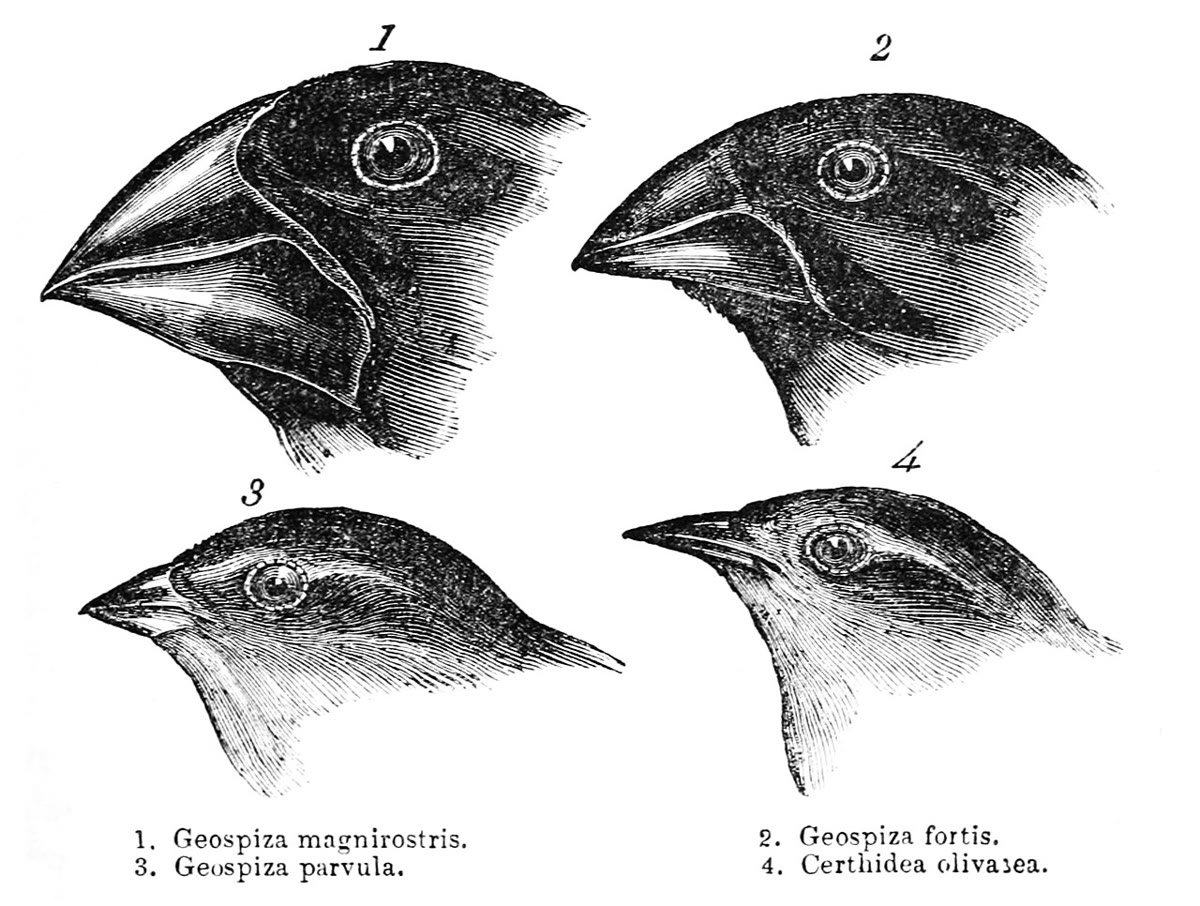
\includegraphics[width=0.44\linewidth]{images/book2/finches-gould.jpg}\hspace{0.04\linewidth}
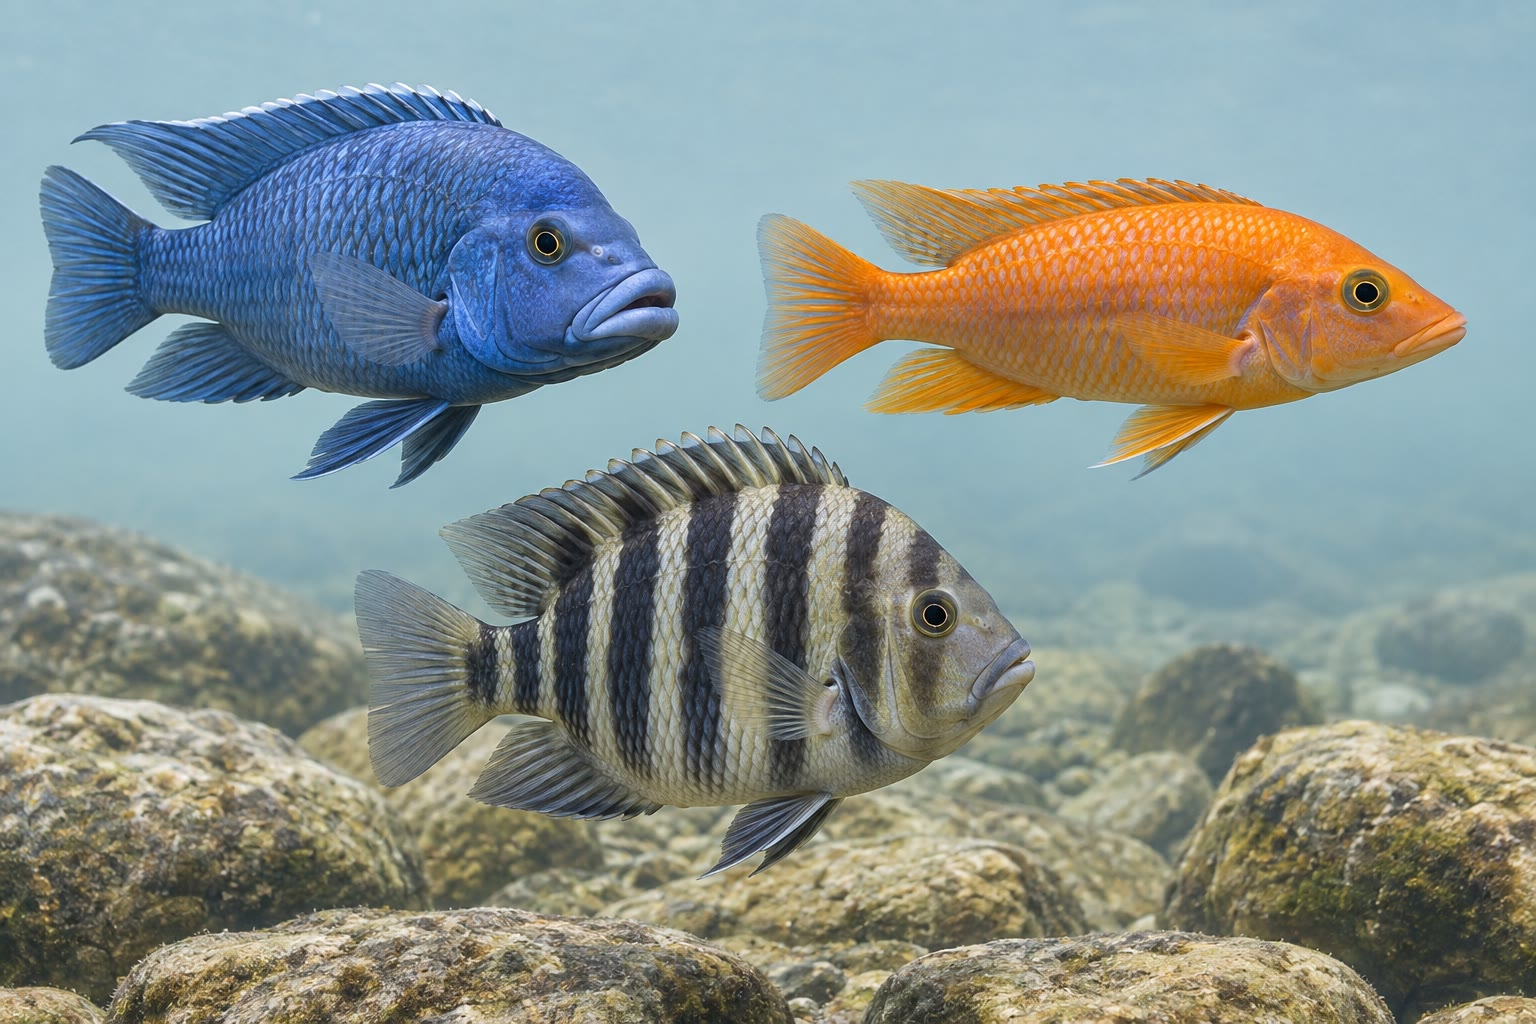
\includegraphics[width=0.44\linewidth]{images/book4/ai/b4-23-cichlids.jpg}

{\small Dos radiaciones. Izquierda: los pinzones de Darwin dibujados por
Gould en 1845, un colonizador convertido en muchos, que se distinguen por
sus picos. Derecha: cíclidos de un lago africano, cientos de especies a
partir de unos pocos fundadores, cada una con su propia boca y su propia
dieta.}
\end{omfigure}

\section{La macroevolución: la visión a largo plazo}

\begin{proposition}[Ritmo y modo]\label{prop:b2:speciation:tempo}
\index{equilibrio puntuado}\index{gradualismo}\index{extinción masiva}
En unas pocas decenas de generaciones, la polilla cambió de color y el
pinzón de pico; a lo largo de millones de años, el registro fósil muestra
linajes que apenas cambian durante largos periodos y que después, en un
instante geológico de unos pocos miles de años, son sustituidos por un
descendiente distinto --- el \emph{\omterm{prop:b2:speciation:tempo}{equilibrio puntuado}}, que es el aspecto
que tiene una \omterm{prop:b2:speciation:modes}{especiación alopátrica} en pequeñas poblaciones periféricas
seguida de su expansión cuando se muestrea cada cien mil años ---; y
muestra otros linajes, entre ellos los caballos, que cambian gradualmente
a lo largo de decenas de especies. Por encima de la especie, el registro
es de renovación: la mayoría de las especies duran de uno a diez millones
de años, la tasa de \emph{extinción de fondo} es de alrededor de una
especie de cada millón por año, y cinco veces --- a finales del
Ordovícico, el Devónico, el Pérmico (cuando desaparecieron nueve décimas
partes de las especies marinas), el Triásico y el Cretácico --- una
\emph{\omterm{prop:b2:speciation:tempo}{extinción masiva}} eliminó la mayor parte de lo que vivía en unos
pocos cientos de miles de años y reinició la partida, con los
supervivientes radiando hacia los nichos vaciados: los mamíferos hacia el
mundo de los dinosaurios tras el asteroide de hace 66 millones de años.
La macroevolución es el dibujo que ha trazado la microevolución de este
capítulo y del anterior, funcionando durante muchísimo tiempo e
interrumpida por catástrofes.
\end{proposition}

\begin{example}[Ritmos comparados]\label{ex:b2:speciation:rates}
La selección sobre los pinzones cambió la profundidad del pico un
\qty{4}{\%} en una generación; toda la radiación de las Galápagos, catorce
especies a partir de un fundador, llevó dos millones de años; la
diferencia de tamaño corporal entre un ratón y un elefante, de alrededor de
$10^{5}$, podría producirse con una selección de la intensidad de la de los
pinzones en unos pocos cientos de generaciones ---
y el registro muestra que llevó cuarenta millones de años. La paradoja se
resuelve advirtiendo que la selección rara vez empuja en el mismo sentido
durante mucho tiempo: se invierte con el clima, como ocurrió en Daphne
Major el año siguiente a la sequía, y la \omterm{prop:b2:population-genetics:kinds}{selección estabilizadora} mantiene
a la mayoría de los linajes donde están. El cambio sostenido es raro, y por
eso la especiación, que lo necesita, es lenta --- y por eso, cuando el
mundo cambia deprisa, como en el \cref{ch:b2:global-change}, se pierden
los linajes que no pueden seguirlo.
\end{example}

\section{Ejercicios}

\begin{exercise}[$\star$]\label{exo:b2:speciation:1}
Enúnciese el \omterm{def:b2:speciation:species}{concepto biológico de especie} y dense tres casos en los que
no puede aplicarse, con el concepto que se usa en su lugar.
\end{exercise}

\begin{exercise}[$\star$]\label{exo:b2:speciation:2}
Clasifíquense como precigóticos o poscigóticos: dos ranas que se
reproducen en meses distintos; una mula; un espermatozoide de erizo de mar
que no puede unirse al óvulo de otra especie; plantas híbridas vigorosas
pero cuyas \omterm{def:b2:angiosperm-reproduction:seed}{semillas} no germinan; dos grillos con cantos distintos.
\end{exercise}

\begin{exercise}[$\star$]\label{exo:b2:speciation:3}
Defínanse la \omterm{prop:b2:speciation:modes}{especiación alopátrica}, la peripátrica, la simpátrica y la
parapátrica, con un ejemplo de cada una.
\end{exercise}

\begin{exercise}[$\star$]\label{exo:b2:speciation:4}
Enúnciense los cuatro resultados de la \omterm{thm:b2:speciation:lv}{competencia de Lotka--Volterra} y la
condición de coexistencia estable, expresada con palabras.
\end{exercise}

\begin{exercise}[$\star\star$]\label{exo:b2:speciation:5}
Con $K_1 = 1000$, $K_2 = 800$, $\alpha = 0.5$, $\beta = 0.6$,
calcúlense las densidades de equilibrio y compruébese que cada especie
puede invadir la capacidad de carga de la otra.
\end{exercise}

\begin{exercise}[$\star\star$]\label{exo:b2:speciation:6}
Con $K_1 = 1000$, $K_2 = 800$, $\alpha = 1.5$, $\beta = 0.3$, ¿qué
especie gana, y por qué? ¿Y si $\alpha = 1.5$ y $\beta = 1.5$?
\end{exercise}

\begin{exercise}[$\star\star$]\label{exo:b2:speciation:7}
Surge un tetraploide en una población \omterm{def:b2:meiosis-heredity:meiosis}{diploide}. Dense los números
cromosómicos de sus gametos, de un cruzamiento con el \omterm{def:b2:meiosis-heredity:meiosis}{diploide} y de los
gametos de ese híbrido, y explíquese por qué el tetraploide queda aislado
de inmediato. ¿Por qué, aun así, no suele persistir?
\end{exercise}

\begin{exercise}[$\star\star$]\label{exo:b2:speciation:8}
Dos poblaciones han fijado cada una 10 sustituciones desde que se
separaron, y cada par de \omterm{def:b2:meiosis-heredity:vocabulary}{alelos} nuevos de los dos lados es incompatible
con probabilidad $0.01$. Calcúlese el número esperado de
incompatibilidades ahora, y después de 30 sustituciones en cada una. ¿Qué
predice esto sobre la relación entre el aislamiento y el tiempo?
\end{exercise}

\begin{exercise}[$\star\star$]\label{exo:b2:speciation:9}
Calcúlese la anchura de una \omterm{prop:b2:speciation:reinforcement}{zona híbrida} para una dispersión $\sigma =
\qty{2}{km}$ por generación y una desventaja de los híbridos $s = 0.05$, y
para $\sigma = \qty{0.3}{km}$ y $s = 0.4$. ¿Qué zona tiene más
probabilidades de terminar en refuerzo, y por qué?
\end{exercise}

\begin{exercise}[$\star\star\star$]\label{exo:b2:speciation:10}
Dos especies de pinzones compiten por \omterm{def:b2:angiosperm-reproduction:seed}{semillas} con $\alpha = \beta = 0.9$ y
$K_1 = K_2 = 500$. ¿Coexisten? El \omterm{prop:b2:speciation:displacement}{desplazamiento de caracteres} reduce
$\alpha$ y $\beta$ a $0.4$: vuélvase a calcular el equilibrio. Explíquese
en términos de isoclinas lo que ha hecho el desplazamiento.
\end{exercise}

\begin{exercise}[$\star\star\star$]\label{exo:b2:speciation:11}
Los Grant hallaron que, tras la sequía de 2004, la profundidad media del
pico del pinzón terrestre mediano bajó \qty{0.7}{mm} con $h^{2} = 0.7$,
y que los supervivientes tenían picos \qty{1}{mm} más pequeños que la
población. Compruébese la respuesta con la \omterm{thm:b2:population-genetics:heritability}{ecuación del criador}, y
explíquese por qué fue la presencia del pinzón terrestre grande, y no solo
la sequía, lo que determinó el sentido del cambio.
\end{exercise}

\begin{exercise}[$\star\star\star$]\label{exo:b2:speciation:12}
``Las especies se hacen por accidente y se mantienen por selección.''
Discútase, con el modelo de dos loci, el refuerzo y el papel de la
geografía.
\end{exercise}

\section{Problema: dos pinzones en una isla}

\begin{problem}[{Problema de fin de semana --- un pinzón residente se
encuentra con un invasor: su competencia analizada en el plano de fases,
el desplazamiento del pico del residente predicho con la ecuación del
criador y el aislamiento entre ambos medido frente a una zona híbrida,
hasta llegar a las densidades de equilibrio, el desplazamiento del pico y
la anchura de la clina}]
\label{pb:b2:speciation:1}
Especie residente 1: $K_1 = 1200$, $r_1 = 0.5$ por año; especie invasora
2: $K_2 = 400$. Antes del desplazamiento, $\alpha = 0.9$, $\beta =
0.3$; una sequía reduce a la mitad ambas capacidades de carga durante un
año. Profundidad del pico de la especie 1: media de \qty{9.5}{mm},
desviación típica de
\qty{0.8}{mm}, $h^{2} = 0.7$. Parámetros de la \omterm{prop:b2:speciation:reinforcement}{zona híbrida}: $\sigma =
\qty{0.5}{km}$, $s = 0.2$.

\medskip
\noindent\textbf{Parte I --- La invasión.}
\begin{enumerate}
  \item Escríbanse las dos isoclinas y sus puntos de corte con los ejes.
  \item ¿Puede la especie 2 invadir la especie 1 en $K_1$? ¿Puede la
        especie 1 invadir la especie 2 en $K_2$? Conclúyase sobre el
        resultado.
  \item Calcúlense las densidades de equilibrio.
  \item Calcúlese $\mathrm{d}N_1/\mathrm{d}t$ en el momento en que llega
        la especie 2, con $N_2 = 20$ y $N_1 = 1200$. ¿Qué significa su
        signo?
  \item Durante la sequía, las dos $K$ se reducen a la mitad. Vuélvase a
        calcular el equilibrio e indíquese qué les ocurre a los efectivos
        de cada especie.
  \item ¿Por qué el efecto del invasor sobre el residente ($\alpha = 0.9$)
        es mayor que el del residente sobre el invasor ($\beta = 0.3$)?
\end{enumerate}

\medskip
\noindent\textbf{Parte II --- El desplazamiento.}
Durante la sequía, los individuos residentes de pico más grande son los
que más compiten con el invasor y mueren: los supervivientes tienen un
pico medio de \qty{9.0}{mm}.
\begin{enumerate}[resume]
  \item Calcúlense el diferencial de selección y la respuesta.
  \item Dese el pico medio de la generación siguiente.
  \item Tras el desplazamiento, $\alpha$ baja a $0.5$. Vuélvase a calcular
        el equilibrio (con las $K$ originales).
  \item Explíquese qué le ha hecho el desplazamiento a la isoclina de la
        especie 1.
  \item Si una selección de esta intensidad actuara todos los años,
        ¿cuántos años se tardaría en desplazar el pico \qty{2}{mm}? ¿Por
        qué no ocurre así?
  \item Compárese con la edad de dos millones de años de la radiación y
        coméntese.
\end{enumerate}

\medskip
\noindent\textbf{Parte III --- El aislamiento.}
Las dos especies pueden hibridarse; los híbridos tienen picos intermedios
y una eficacia $1 - s$.
\begin{enumerate}[resume]
  \item Nómbrense la barrera precigótica que mantiene raras las
        hibridaciones en los pinzones de Darwin y un coste poscigótico de
        los híbridos.
  \item Calcúlese la anchura de una \omterm{prop:b2:speciation:reinforcement}{zona híbrida} entre ellas para $\sigma
        = \qty{0.5}{km}$, $s = 0.2$.
  \item La isla mide \qty{1}{km} de un extremo a otro. ¿Qué implica eso?
  \item Explíquese cómo avanzaría el refuerzo y sobre qué carácter
        actuaría.
  \item Dos poblaciones del residente en islas distintas han fijado cada
        una 15 sustituciones desde que se separaron; los pares son
        incompatibles con probabilidad $0.005$. Calcúlense las
        incompatibilidades esperadas e indíquese si son especies.
  \item ¿Coincidirían el \omterm{def:b2:speciation:species}{concepto biológico de especie}, el concepto
        morfológico y el concepto filogenético sobre las dos poblaciones
        insulares? Explíquese.
\end{enumerate}

\medskip
\noindent\textbf{Parte IV --- La visión a largo plazo.}
\begin{enumerate}[resume]
  \item Si una especie dura por término medio 5 millones de años, ¿cuál es
        la tasa de extinción de fondo por especie y por año? Para una
        biota de 10 millones de especies, ¿cuántas extinciones por año?
  \item La tasa de extinción actual se estima entre 100 y 1000 veces la de
        fondo. ¿Cuántas especies por año son?
  \item Una \omterm{prop:b2:speciation:tempo}{extinción masiva} elimina el \qty{75}{\%} de las especies en
        \num{100000} años. Compárese su tasa con la actual.
  \item Explíquese en una frase por qué los supervivientes de una
        \omterm{prop:b2:speciation:tempo}{extinción masiva} experimentan una radiación.
  \item Un linaje del registro cambia poco durante 3 millones de años y
        después es sustituido en \num{20000} años por un descendiente
        distinto. Nómbrese el patrón e indíquese el modo de especiación
        que lo produce.
  \item Con el \qty{4}{\%} por generación de los pinzones, ¿cuántas
        generaciones de selección sostenida duplicarían la profundidad del
        pico? ¿Por qué el registro fósil muestra que estos cambios llevan
        millones de años?
  \item Enúnciese el resultado: el resultado y el equilibrio de la
        competencia antes y después del desplazamiento, el desplazamiento
        del pico en una generación y la anchura de la \omterm{prop:b2:speciation:reinforcement}{zona híbrida}.
\end{enumerate}
\end{problem}
